\documentclass{article}

\usepackage{graphicx} % Required for inserting images
\usepackage{amsmath, amssymb, amsthm} % For better use of Math expressions
\usepackage{hyperref} % for adding hyperlinks to the document. 
\usepackage{comment}
\usepackage{marginnote} % Adding notes to the margin of the document
\reversemarginpar % Optional: to switch margin sides
\usepackage{xcolor} % For creating the the colorbox
% For creating tcolorboxes. 
\usepackage{tikz}
\usepackage[most]{tcolorbox}
\usepackage{lipsum}
\usepackage{enumitem} % for enumerating items with letters from the alphabet.
\usepackage{tabularx} % Enables tables with flexible-with columns
\usepackage{etoolbox} % For custom labels and logic.
\usepackage{array} % Extend column definitions in tables
\usepackage{witharrows} % for adding arrows

% ==== Customization ====
\usepackage [letterpaper, top=1.0in, bottom=1.0in, left=1.0in, right=1.0in, heightrounded]{geometry} % Margins of the document. 
\renewcommand{\baselinestretch}{1.2} % space line length
\setlength{\parindent}{0pt} % Change the size of the tab
\setlength{\parskip}{0.8em} %Change the size between paragraphs

\title{\textbf{Cal 2 - Exam Question 34}}
\author{Diana Guan}
\date{March 2026}


% ==== Custom Macros ====
% Create a general counter that resets automatically per question
\newcounter{solutionMainStep}
\newcounter{solutionSubStep}[solutionMainStep]

% Define a macro that takes question number, summary of step on (left), and explanation of the step on (right). 
\renewcommand{\thesolutionSubStep}{\arabic{solutionMainStep}.\arabic{solutionSubStep}}
\newcommand{\deflink}[2]{\hyperlink{def:#1}{\textcolor{blue}{\underline{#2}}}}
\newcommand{\defanchor}[1]{\hypertarget{def:#1}{}}
\newcommand{\questionanchor}[1]{\hypertarget{q:#1}{}}
\newcommand{\qdeflink}[2]{\hypertarget{q:#1}{}\deflink{#1}{#2}}
\newcommand{\backtoterm}[2]{\hyperlink{q:#1}{\textbf{#2}}}

% Macro for main step 
\newcommand{\mainStep}[2]{%
    \refstepcounter{solutionMainStep}
    \setcounter{solutionSubStep}{0} % reset sub steps.
    \label{a-#1:\arabic{solutionMainStep}}% adding a label to the macro for later reference.
    % Code to organize and display the bubbles
    \begin{tcolorbox}[
        breakable,
        colback = gray!5!white, 
        colframe = gray!80!black, 
        boxrule = 0.5pt,
        arc = 2mm, 
        left=0pt, right=0pt, top=2pt, bottom=2pt,
        before skip=2pt, after skip = 2pt,
        enhanced]
        \textbf{Step \arabic{solutionMainStep}:} \textbf{\small #2}
    \end{tcolorbox}
}

% Macro for substep (e.g., "Step 1.1:")
\newcommand{\solutionStep}[3]{%
    \refstepcounter{solutionSubStep}
    \label{a-#1:\arabic{solutionMainStep}.\arabic{solutionSubStep}}% adding a label to the macro for later reference.
    % Code to organize and display the bubbles
    \begin{tcolorbox}[
        breakable,
        colback = gray!5!white,
        colframe = gray!80!black,
        boxrule = 0.5pt,
        arc = 2mm,
        left=0pt, right=0pt, top=2pt, bottom=2pt,
        before skip=2pt, after skip=2pt,
        enhanced]
        \begin{tabularx}{\textwidth}{>{\raggedright\arraybackslash}p{5cm} X}
            \textbf{Step \arabic{solutionMainStep}.\arabic{solutionSubStep}:}\\
            \textbf{\small #2} & #3
        \end{tabularx}
    \end{tcolorbox}
}

% To reference a step:
% Use \ref{a-<question>:<step>} anywhere in the text.
% Example: \ref{a-2:1.2} refers to Step 1.2 of Question 2.

% ==== Beginning of Document ==== 
\begin{document}

\maketitle

    %Question 34
    \questionanchor{34}
    \section*{Question 34}
    Evaluate
    \[
    \displaystyle\int \frac{x^2}{(4-x^2)^{\frac{3}{2}}}\, dx.
    \]
    
    % Possible answers
    \begin{enumerate}[label = \alph*.]
        \item $\displaystyle \frac{2x}{\sqrt{4-x^2}} - 2\sin^{-1}\!\left(\frac{x}{2}\right) + C$
        \item $\displaystyle \frac{x}{\sqrt{4-x^2}} - \sin^{-1}\!\left(\frac{x}{2}\right) + C$
        \item $\displaystyle \frac{4}{\sqrt{4-x^2}} - 2\sin^{-1}\!\left(\frac{x}{2}\right) + C$
        \item I do not know
    \end{enumerate}

    % Beginning of Solution Box
     \begin{tcolorbox}[breakable, colback= blue!5!white, colframe= blue!50!black, title=\textbf{Solution: b) $\displaystyle \frac{x}{\sqrt{4-x^2}} - \sin^{-1}\!\left(\frac{x}{2}\right) + C$}]

        % Step-by-step modular solution. 
        \textbf{This question is asking you to:} Compute an \qdeflink{antiderivative}{antiderivative} by rewriting the
        \qdeflink{denominator}{denominator} into a form that matches a standard \qdeflink{trig-sub}{trigonometric substitution}
        pattern, then substitute back to write the final answer in terms of $x$.
        
        % ------- Start here adding the step-by-step solution --------
        
        % Step 1
        \mainStep{1}{Rewrite the denominator $(4-x^2)^{\frac{3}{2}}$.}

        % Step 1.1
        \solutionStep{1}{Identify the \qdeflink{denominator}{denominator}}{
        In
        \[
        \frac{x^2}{(4-x^2)^\frac{3}{2}},
        \]
        the denominator is the bottom part:
        \[
        (4-x^2)^{\frac{3}{2}}.
        \]
        }

        % Step 1.2
        \solutionStep{1}{Rewrite \qdeflink{frac-exp}{fractional exponents}}{
        Since the denominator is complicated, we want to simplify it by rewriting the power.
        \[
        (4-x^2)^{\frac{3}{2}}
        \]
        has a fractional exponent, and we can rewrite fractional exponents using:
        \[
        a^{\frac{m}{n}}=\sqrt[n]{a^m}=\left(\sqrt[n]{a}\right)^m,\qquad \deflink{square-root}{\sqrt{a}}=a^{\frac{1}{2}}.
        \]
        }
        
        % Step 1.3
        \solutionStep{1}{Rewrite the power $\frac{3}{2}$}{
        \[
        \hspace*{-3em}
        \begin{array}{@{}r@{\hspace{1.25em}}l@{}}
        \text{Rewrite } \frac{3}{2}=\frac{1}{2}\cdot 3
        &
        (4-x^2)^{\tikz[remember picture,baseline=(expA.base)] \node[fill=yellow,inner sep=1pt](expA){$\frac{3}{2}$};}
        = (4-x^2)^{\tikz[remember picture,baseline=(expB.base)] \node[fill=yellow,inner sep=1pt](expB){$\frac{1}{2}\cdot 3$};}
        \\[2.2ex]
        \text{Use } a^{bc}=(a^b)^c
        &
        (4-x^2)^{\tikz[remember picture,baseline=(expC.base)] \node[fill=yellow,inner sep=1pt](expC){$\frac{1}{2}\cdot 3$};}
        =
        \left((4-x^2)^{\tikz[remember picture,baseline=(expD.base)] \node[fill=yellow,inner sep=1pt](expD){$\frac{1}{2}$};}\right)^3
        \\[2.2ex]
        \text{Rewrite } (4-x^2)^{\frac{1}{2}} \text{ as a \qdeflink{square-root}{square root}}
        &
        \left((4-x^2)^{\tikz[remember picture,baseline=(expE.base)] \node[fill=yellow,inner sep=1pt](expE){$\frac{1}{2}$};}\right)^3
        =
        \left(\tikz[remember picture,baseline=(expF.base)] \node[fill=yellow,inner sep=1pt](expF){$\sqrt{4-x^2}$};\right)^3
        \end{array}
        \]
        \begin{tikzpicture}[remember picture,overlay]
            \draw[->,>=stealth,bend left=20] ([yshift=7pt]expA.north) to ([yshift=7pt]expB.north);
            \draw[->,>=stealth,bend left=10] ([yshift=6pt]expC.north) to ([yshift=6pt]expD.north);
            \draw[->,>=stealth,bend left=8] ([yshift=6pt]expE.north) to ([yshift=6pt]expF.north);
        \end{tikzpicture}
        }

        % Step 2
         \mainStep{1}{Set up \deflink{trig-sub}{trigonometric substitution}.}

        % Step 2.1
        \solutionStep{1}{Notice the trig substitution pattern}{
        Right now the denominator still looks complicated, so we want to simplify it more.
        The denominator contains
        \[
        \sqrt{4-x^2},
        \]
        and this looks like the \deflink{trig-sub}{trigonometric substitution} pattern
        \[
        \sqrt{a^2-x^2}.
        \]
        }

        % Step 2.2
        \solutionStep{1}{Define the symbols}{
        $a$: \deflink{constant}{constant},\quad $x$: \deflink{variable}{variable},\quad $\theta$: angle.
        }

        % Step 2.3
        \solutionStep{1}{Trigonometric pattern $\sqrt{a^2-x^2}$}{
        When we encounter the pattern
        \[
        \sqrt{a^2-x^2},
        \]
        we let
        \[
        x=a\sin\theta.
        \]
        }

        % Step 2.4
        \solutionStep{1}{Rewrite the fraction $\sqrt{a^2-x^2}$}{
        \[
        \begin{aligned}
        \text{Substitute } x=a\sin\theta
        \qquad &
        \sqrt{a^2-\tikz[remember picture,baseline=(subX.base)] \node[fill=yellow,inner sep=1pt](subX){$x$};^2}
        =
        \sqrt{a^2-(\tikz[remember picture,baseline=(subASin.base)] \node[fill=yellow,inner sep=1pt](subASin){$a\sin\theta$};)^2}
        \end{aligned}
        \]
        \begin{tikzpicture}[remember picture,overlay]
            \draw[->,>=stealth,bend left=20] ([yshift=7pt]subX.north) to ([yshift=7pt]subASin.north);
        \end{tikzpicture}
        }

        % Step 2.5
        \solutionStep{1}{Simplify $\sqrt{a^2-(a\sin\theta)^2}$}{
        \[
        \begin{array}{@{}r@{\hspace{1.25em}}l@{}}
        \text{Use \deflink{prod-power}{Power of a Product Rule},}
        &
        (a\colorbox{yellow}{$b$})^2=a^2\colorbox{yellow}{$b$}^2
        \\[1.2ex]
        \text{Substitute } b=\sin\theta,
        &
        (a\colorbox{yellow}{$\sin\theta$})^2=a^2(\colorbox{yellow}{$\sin\theta$})^2
        \\[1.2ex]
        &
        \hspace{-4.5em}
        \sqrt{a^2-\colorbox{yellow}{$(a\sin\theta)^2$}}
        = \sqrt{a^2-\colorbox{yellow}{$a^2(\sin\theta)^2$}}
        \end{array}
        \]
        }

        % Step 2.6
        \solutionStep{1}{Trig substitution summary}{
        $\begin{aligned}[t]
        \text{For pattern } \sqrt{a^2-x^2}, \text{ let } x &= a\sin\theta\\
        \sqrt{a^2-x^2} &= \sqrt{a^2-a^2(\sin\theta)^2}
        \end{aligned}$
        }

        % Step 3
        \mainStep{1}{Rewrite $\sqrt{4-x^2}$ using trigonometric substitution.}

        % Step 3.1
        \solutionStep{1}{Identify $a$ and $x$ in $\sqrt{4-x^2}$}{
        \[
        \begin{array}{@{}r@{\hspace{0.4em}}l@{\hspace{1.25em}}r@{\hspace{0.35em}}c@{\hspace{0.35em}}l@{}}
        \text{Rewrite } 4=2\cdot 2=
        &
        2^2
        &
        \sqrt{\tikz[remember picture,baseline=(step3A.base)] \node[fill=yellow,inner sep=1pt](step3A){$4$};-x^2}
        &
        =
        &
        \sqrt{\tikz[remember picture,baseline=(step3B.base)] \node[fill=yellow,inner sep=1pt](step3B){$2^2$};-x^2}
        \\[1.2ex]
        &
        \text{Let}
        &
        \sqrt{2^2-x^2}
        &
        =
        &
        \sqrt{a^2-x^2}
        \\[1.2ex]
        &
        &
        a
        &
        =
        &
        \colorbox{yellow}{$2$}
        \\[1.2ex]
        &
        &
        x
        &
        =
        &
        \colorbox{yellow}{$a$}\sin\theta = \colorbox{yellow}{$2$}\sin\theta
        \end{array}
        \]
        \begin{tikzpicture}[remember picture,overlay]
            \draw[->,>=stealth,bend left=20] ([yshift=7pt]step3A.north) to ([yshift=7pt]step3B.north);
        \end{tikzpicture}
        }

        % Step 3.2
        \solutionStep{1}{Substitute $a=2$, $x=2\sin\theta$ into the fraction}{
        $\begin{aligned}[t]
        \sqrt{a^2-x^2}
        &= \sqrt{a^2-a^2(\sin\theta)^2}\\
        \sqrt{2^2-x^2}
        &= \sqrt{2^2-2^2(\sin\theta)^2}
        \end{aligned}$
        }

        % Step 4
        \mainStep{1}{Simplify $\sqrt{2^2-2^2(\sin\theta)^2}$.}

        % Step 4.1
        \solutionStep{1}{Replace $2^2=4$}{
        \[
        \begin{array}{@{}r@{\hspace{1.25em}}l@{}}
        \text{Replace } 2^2=4
        &
        \sqrt{\colorbox{yellow}{$2^2$}-\colorbox{yellow}{$2^2$}(\sin\theta)^2}
        = \sqrt{\colorbox{yellow}{$4$}-\colorbox{yellow}{$4$}(\sin\theta)^2}
        \end{array}
        \]
        }

        % Step 4.2
        \solutionStep{1}{Factor out $4$}{
        \[
        \begin{array}{@{}r@{\hspace{1.25em}}l@{}}
        \text{Rewrite } 4=4\cdot 1
        &
        \colorbox{yellow}{$4$}-4(\sin\theta)^2
        = \colorbox{yellow}{$4(1)$}-4((\sin\theta)^2)
        \\[1.2ex]
        \text{Factor out } 4
        &
        \colorbox{yellow}{$4$}-\colorbox{yellow}{$4$}(\sin\theta)^2
        = \colorbox{yellow}{$4$}(1-(\sin\theta)^2)
        \end{array}
        \]
        }

        % Step 4.3
        \solutionStep{1}{Simplify $1-(\sin\theta)^2$}{
        \[
        \hspace*{-4.5em}
        \begin{array}{@{}r@{\hspace{1.25em}}r@{\hspace{0.35em}}c@{\hspace{0.35em}}l@{}}
        \text{By } (\sin\theta)^2=\sin^2\theta\text{,}
        &
        4(1-\colorbox{yellow}{$(\sin\theta)^2$})
        &
        =
        &
        4(1-\colorbox{yellow}{$\sin^2\theta$})
        \\[1.2ex]
        \text{By \qdeflink{pyth-id}{Pythagorean identity},}
        &
        1-\sin^2\theta
        &
        =
        &
        \cos^2\theta
        \\[1.2ex]
        \text{Substitute the Pythagorean identity,}
        &
        4(\colorbox{yellow}{$1-\sin^2\theta$})
        &
        =
        &
        4(\colorbox{yellow}{$\cos^2\theta$})
        \end{array}
        \]
        }

        % Step 4.4
        \solutionStep{1}{Summary}{
        $\begin{aligned}[t]
        \sqrt{4-x^2}
        &= \sqrt{2^2-x^2}\quad \text{from \hyperref[a-1:3.1]{Step 3.1}}\\
        &= \sqrt{2^2-2^2(\sin\theta)^2}\quad \text{from \hyperref[a-1:3.2]{Step 3.2}}\\
        &= \sqrt{4(1-\sin^2\theta)}\quad \text{from \hyperref[a-1:4.1]{Step 4.1} and \hyperref[a-1:4.2]{Step 4.2}}\\
        &= \sqrt{4\cos^2\theta}\quad \text{from \hyperref[a-1:4.3]{Step 4.3}}
        \end{aligned}$
        }

        % Step 5
        \mainStep{1}{Compute $(4-x^2)^{\frac{3}{2}}$ after substitution.}

        % Step 5.1
        \solutionStep{1}{Substitute into $\left(\sqrt{4-x^2}\right)^3$}{
        \[
        \hspace*{-2.5em}
        \begin{array}{@{}r@{\hspace{1.25em}}l@{}}
        \text{From \hyperref[a-1:1.3]{Step 1.3},}
        &
        (4-x^2)^{\frac{3}{2}}=\left(\sqrt{4-x^2}\right)^3
        \\[1.5ex]
        \text{Substitute } \sqrt{4-x^2}=\sqrt{4\cos^2\theta}
        &
        \left(\sqrt{\tikz[remember picture,baseline=(step5A.base)] \node[fill=yellow,inner sep=1pt](step5A){$4-x^2$};}\right)^3
        =
        \left(\sqrt{\tikz[remember picture,baseline=(step5B.base)] \node[fill=yellow,inner sep=1pt](step5B){$4\cos^2\theta$};}\right)^3
        \end{array}
        \]
        \begin{tikzpicture}[remember picture,overlay]
            \draw[->,>=stealth,bend left=10] ([yshift=7pt]step5A.north) to ([yshift=7pt]step5B.north);
        \end{tikzpicture}
        }
        
        % Step 5.2
        \solutionStep{1}{Simplify $\sqrt{4\cos^2\theta}$}{
        \[
        \begin{array}{@{}r@{\hspace{1.25em}}l@{}}
        \text{Since }\text{\hyperlink{def:sqrt-rule}{\textcolor{blue}{\(\sqrt{ab}=\sqrt{a}\sqrt{b}\)}}}\text{,}
        &
        \sqrt{\tikz[remember picture,baseline=(step52A.base)] \node[fill=yellow,inner sep=1pt](step52A){$4$};\,\cos^2\theta}
        =
        \tikz[remember picture,baseline=(step52B.base)] \node[fill=yellow,inner sep=1pt](step52B){$\sqrt4$};\,\sqrt{\cos^2\theta}
        \\[2.0ex]
        \text{$\sqrt4=2$}
        &
        \tikz[remember picture,baseline=(step52C.base)] \node[fill=yellow,inner sep=1pt](step52C){$\sqrt4$};\,\sqrt{\cos^2\theta}
        =
        \tikz[remember picture,baseline=(step52D.base)] \node[fill=yellow,inner sep=1pt](step52D){$2$};\,\sqrt{\cos^2\theta}
        \end{array}
        \]
        \begin{tikzpicture}[remember picture,overlay]
            \draw[->,>=stealth,bend left=10] ([yshift=7pt]step52A.north) to ([yshift=7pt]step52B.north);
            \draw[->,>=stealth,bend left=8] ([yshift=6pt]step52C.north) to ([yshift=6pt]step52D.north);
        \end{tikzpicture}
        }

        % Step 5.4
        \solutionStep{1}{Rewrite $\sqrt{4\cos^2\theta}$ as $2|\cos\theta|$}{
        \[
        \begin{array}{@{}r@{\hspace{1.25em}}l@{}}
        \text{Use } \sqrt{u^2}=|u|
        &
        \sqrt{\cos^2\theta}=|\cos\theta|
        \\[1.2ex]
        \text{Multiply both sides by } 2
        &
        \colorbox{yellow}{$2$}\sqrt{\cos^2\theta}
        =
        \colorbox{yellow}{$2$}|\cos\theta|
        \end{array}
        \]
        }


        % Step 5.5
        \solutionStep{1}{Cube both sides}{
        \[
        \begin{array}{@{}r@{\hspace{1.25em}}l@{}}
        \text{Cube both sides}
        &
        \left(\sqrt{4\cos^2\theta}\right)^{\colorbox{yellow}{$3$}}
        =
        (2|\cos\theta|)^{\colorbox{yellow}{$3$}}
        \\[1.2ex]
        \text{Use } (ab)^3=a^3b^3
        &
        (2|\cos\theta|)^3
        =
        \colorbox{yellow}{$2^3$}|\cos\theta|^3
        \\[1.2ex]
        \text{Simplify } 2^3
        &
        \left(\sqrt{4\cos^2\theta}\right)^3
        =
        \colorbox{yellow}{$8$}|\cos\theta|^3
        \end{array}
        \]
        }

        % Step 5.6
        \solutionStep{1}{Remove the absolute value}{
        \[
        \begin{array}{@{}r@{\hspace{1.25em}}l@{}}
        \text{For } x=2\sin\theta\text{, we take }
        0\le \theta\le \frac{\pi}{2}
        &
        \cos\theta\ge 0
        \\[1.2ex]
        \text{So } |\cos\theta|=\cos\theta
        &
        8|\cos\theta|^3=8\cos^3\theta
        \end{array}
        \]
        }

        \solutionStep{1}{Summary}{
        \[
        \begin{aligned}[t]
        \sqrt{4\cos^2\theta}
        &= 2\sqrt{\cos^2\theta}\quad \text{from \hyperref[a-1:5.2]{Step 5.2}}\\
        2\sqrt{\cos^2\theta}
        &= 2|\cos\theta|\quad \text{from \hyperref[a-1:5.3]{Step 5.3}}\\
        \left(\sqrt{4\cos^2\theta}\right)^3
        &= 8|\cos\theta|^3\quad \text{from \hyperref[a-1:5.4]{Step 5.4}}\\
        (4-x^2)^{\frac{3}{2}}
        &= 8\cos^3\theta\quad \text{from \hyperref[a-1:5.6]{Step 5.6}}
        \end{aligned}
        \]
        }
        
        % Step 6
        \mainStep{1}{Rewrite the \qdeflink{numerator}{numerator} $x^2$.}
        
        % Step 6.1
        \solutionStep{1}{Square both sides}{
        \[
        \begin{array}{@{}r@{\hspace{1.25em}}l@{}}
        \text{Start with the substitution}
        &
        x=2\sin\theta\quad \text{from \hyperref[a-1:3.1]{Step 3.1}}
        \\[1.2ex]
        \text{Square both sides}
        &
        x^2=(2\sin\theta)^2
        \end{array}
        \]
        }
        
        % Step 6.2
        \solutionStep{1}{Apply $(ab)^2=a^2b^2$}{
        \[
        \begin{array}{@{}r@{\hspace{1.25em}}l@{}}
        \text{Let } a=2,\; b=\sin\theta
        &
        (ab)^2=a^2b^2
        \\[1.2ex]
        \text{Substitute into the rule}
        &
        (2\sin\theta)^{\colorbox{yellow}{$2$}}
        =
        2^{\colorbox{yellow}{$2$}}(\sin\theta)^{\colorbox{yellow}{$2$}}
        \end{array}
        \]
        }

        
        % Step 6.3
        \solutionStep{1}{Simplify $2^2(\sin\theta)^2$}{
        \[
        \begin{array}{@{}r@{\hspace{1.25em}}l@{}}
        \text{Compute } 2^2
        &
        2^2=4
        \\[1.2ex]
        \text{By \qdeflink{notation}{square of trigonometric functions}}
        &
        (\sin\theta)^2=\sin^2\theta
        \\[1.2ex]
        \text{Substitute}
        &
        2^2(\sin\theta)^2=4\sin^2\theta
        \\[1.2ex]
        \text{Therefore}
        &
        x^2=4\sin^2\theta
        \end{array}
        \]
        }
        
        % Step 7
        \mainStep{1}{Compute $dx$.}
        
        % Step 7.1
        \solutionStep{1}{Differentiate $x=2\sin\theta$}{
        \[
        \hspace*{-4em}
        \begin{array}{@{}r@{\hspace{1.25em}}l@{}}
        \text{Start with the substitution}
        &
        x=2\sin\theta\quad \text{from \hyperref[a-1:3.1]{Step 3.1}}
        \\[1.2ex]
        \text{Differentiate both sides with respect to } \theta
        &
        \frac{dx}{d\theta}=\frac{d}{d\theta}(2\sin\theta)
        \\[1.2ex]
        \text{Use the \qdeflink{const-mult}{constant multiple rule}}
        &
        \frac{dx}{d\theta}
        =
        \colorbox{yellow}{$2$}\frac{d}{d\theta}(\sin\theta)
        \\[1.2ex]
        \text{Since } \frac{d}{d\theta}(\sin\theta)=\cos\theta
        &
        \frac{dx}{d\theta}
        =
        \colorbox{yellow}{$2$}\cos\theta
        \end{array}
        \]
        }


        % Step 7.2
        \solutionStep{1}{Write $dx$}{
        \[
        \begin{array}{@{}r@{\hspace{1.25em}}l@{}}
        \text{Start with }
        &
        \frac{dx}{d\theta}=2\cos\theta
        \\[1.2ex]
        \text{Multiply both sides by } d\theta
        &
        \colorbox{yellow}{$d\theta$}\left(\frac{dx}{d\theta}\right)
        =
        (2\cos\theta)\colorbox{yellow}{$d\theta$}
        \\[1.2ex]
        \text{So}
        &
        dx=2\cos\theta\, d\theta
        \end{array}
        \]
        }
        
        % Step 8
        \mainStep{1}{Rewrite the integral with substitutions.}
        
        % Step 8.1
        \solutionStep{1}{List substitutions}{
        \[
        \begin{aligned}[t]
            x^2 &= 4\sin^2\theta \quad \text{from \hyperref[a-1:6]{Step 6}}\\
            (4-x^2)^{\frac{3}{2}} &= 8\cos^3\theta \quad \text{from \hyperref[a-1:1]{Step 1} to \hyperref[a-1:5]{Step 5}}\\
            dx &= 2\cos\theta\, d\theta \quad \text{from \hyperref[a-1:7]{Step 7}}
        \end{aligned}
        \]
        }
        
        % Step 8.2
        \solutionStep{1}{Substitute}{
        \[
        \hspace*{-12em}
        \begin{array}{@{}r@{\hspace{1.25em}}l@{}}
        \text{Start with the original integral}
        &
        \displaystyle\int \frac{x^2}{(4-x^2)^{\frac{3}{2}}}\,dx
        \\[1.2ex]
        \text{Substitute the expressions from \hyperref[a-1:8.1]{Step 8.1}}
        &
        \displaystyle\int \frac{x^2}{(4-x^2)^{\frac{3}{2}}}\,dx
        =
        \displaystyle\int
        \frac{\colorbox{yellow}{$4\sin^2\theta$}}{\colorbox{yellow}{$8\cos^3\theta$}}\,
        \colorbox{yellow}{$(2\cos\theta\, d\theta)$}
        \end{array}
        \]
        }
        
        % Step 9
        \mainStep{1}{Simplify the integrand.}
        
        % Step 9.1
        \solutionStep{1}{Multiply constants}{
        \[
        \hspace*{-5em}
        \begin{array}{@{}r@{\hspace{1.25em}}l@{}}
        \text{}
        &
        \displaystyle\int \frac{4\sin^2\theta}{8\cos^3\theta}\,\colorbox{yellow}{$2\cos\theta$}\, d\theta
        =
        \displaystyle\int \frac{4\cdot\colorbox{yellow}{$2$}\sin^2\theta\colorbox{yellow}{$\cos\theta$}}{8\cos^3\theta}\, d\theta
        \\[1.2ex]
        \text{Simplify } 4\cdot 2
        &
        \displaystyle\int \frac{4\cdot2\sin^2\theta\cos\theta}{8\cos^3\theta}\, d\theta
        =
        \displaystyle\int \frac{\colorbox{yellow}{$8$}\sin^2\theta\cos\theta}{8\cos^3\theta}\, d\theta
        \end{array}
        \]
        }
        
        % Step 9.2
        \solutionStep{1}{Cancel 8}{
        \[
        \hspace*{-5em}
        \begin{array}{@{}r@{\hspace{1.25em}}l@{}}
        \text{Cancel the common factor } 8
        &
        \displaystyle\int \frac{\colorbox{yellow}{$8$}\sin^2\theta\cos\theta}{\colorbox{yellow}{$8$}\cos^3\theta}\, d\theta
        =
        \displaystyle\int \frac{\sin^2\theta\cos\theta}{\cos^3\theta}\, d\theta
        \end{array}
        \]
        }
        
        % Step 9.3
        \solutionStep{1}{Cancel $\cos\theta$}{
        \[
        \hspace*{-5em}
        \begin{array}{@{}r@{\hspace{1.25em}}l@{}}
        \text{Rewrite } \cos^3\theta
        &
        \cos^3\theta=\cos^2\theta\cos\theta
        \\[1.2ex]
        \text{Substitute into the denominator}
        &
        \displaystyle\int \frac{\sin^2\theta\cos\theta}{\colorbox{yellow}{$\cos^3\theta$}}\, d\theta
        =
        \displaystyle\int \frac{\sin^2\theta\cos\theta}{\colorbox{yellow}{$\cos^2\theta\cos\theta$}}\, d\theta
        \\[1.2ex]
        \text{Cancel } \cos\theta
        &
        \displaystyle\int \frac{\sin^2\theta\colorbox{yellow}{$\cos\theta$}}{\cos^2\theta\colorbox{yellow}{$\cos\theta$}}\, d\theta
        =
        \displaystyle\int \frac{\sin^2\theta}{\cos^2\theta}\, d\theta
        \end{array}
        \]
        }
        
        % Step 9.4
        \solutionStep{1}{Simplify $\int \frac{\sin^2\theta}{\cos^2\theta}\,d\theta$}{
        \[
        \begin{array}{@{}r@{\hspace{1.25em}}l@{}}
        \text{By definition of tangent,}
        &
        \tan\theta=\dfrac{\sin\theta}{\cos\theta}
        \\[1.2ex]
        \text{Square both sides}
        &
        \tan^2\theta=\dfrac{\sin^2\theta}{\cos^2\theta}
        \\[1.2ex]
        \text{Rewrite the integrand}
        &
        \displaystyle\int \dfrac{\sin^2\theta}{\cos^2\theta}\, d\theta
        =
        \displaystyle\int \tan^2\theta\, d\theta
        \end{array}
        \]
        }
        
        % Step 11
        \mainStep{1}{Integrate in $\theta$.}
        
        % Step 11.1
        \solutionStep{1}{Rewrite the integral}{
        \[
        \hspace*{-7em}
        \begin{array}{@{}r@{\hspace{1.25em}}l@{}}
        \text{Use the \qdeflink{pyth-id}{trigonometry identity}}
        &
        \tan^2\theta=\sec^2\theta-1
        \\[1.2ex]
        \text{Substitute into the integral}
        &
        \displaystyle\int \colorbox{yellow}{$\tan^2\theta$}\, d\theta
        =
        \displaystyle\int \colorbox{yellow}{$(\sec^2\theta-1)$}\, d\theta
        \\[1.2ex]
        \text{By \qdeflink{add-int}{additive property of integrals}}
        &
        \displaystyle\int (\sec^2\theta-1)\, d\theta
        =
        \displaystyle\int \sec^2\theta\, d\theta-\displaystyle\int 1\, d\theta
        \end{array}
        \]
        }
        
        % Step 11.2
        \solutionStep{1}{Integrate}{
        \[
        \hspace*{-3em}
        \begin{array}{@{}r@{\hspace{1.25em}}l@{}}
        \text{Integrate } \sec^2\theta
        &
        \displaystyle\int \sec^2\theta\, d\theta=\tan\theta
        \\[1.2ex]
        \text{Integrate } 1
        &
        \displaystyle\int 1\, d\theta=\theta
        \\[1.2ex]
        \text{Combine the result}
        &
        \displaystyle\int \sec^2\theta\, d\theta-\displaystyle\int 1\, d\theta
        =
        \tan\theta-\theta+C
        \\[1.2ex]
        \text{Therefore}
        &
        \displaystyle\int \tan^2\theta\, d\theta=\tan\theta-\theta+C
        \end{array}
        \]
        }
        
        % Step 12
        \mainStep{1}{Convert $\tan\theta-\theta+C$ back into $x$.}
        
        % Step 12.1
        \solutionStep{1}{Identify what to convert back}{
        We now have the antiderivative in terms of $\theta$, and we want to convert it back to $x$.
        To do that, we need to rewrite both $\tan\theta$ and $\theta$ in terms of $x$.
        }

        % Step 12.2
        \solutionStep{1}{Find $\theta$}{
        \[
        \hspace*{-5em}
        \begin{array}{@{}r@{\hspace{1.25em}}l@{}}
        \text{Start with }
        &
        x=2\sin\theta\quad \text{from \hyperref[a-1:3.1]{Step 3.1}}
        \\[1.2ex]
        \text{Multiply both sides by } \frac{1}{2}
        &
        \colorbox{yellow}{$\frac{1}{2}$}x
        =
        \colorbox{yellow}{$\frac{1}{2}$}2\sin\theta
        \\[1.2ex]
        \text{$\frac{1}{2}\cdot 2=1$}
        &
        \frac{x}{2}=\sin\theta
        \\[1.2ex]
        \text{Apply } \qdeflink{inv-sine}{\sin^{-1}} \text{ to both side of the equation}
        &
        \theta=\sin^{-1}\!\left(\frac{x}{2}\right)
        \end{array}
        \]
        }
        
        % Step 12.3
        \solutionStep{1}{Write the sine ratio}{
        \[
        \hspace*{-4em}
        \begin{array}{@{}r@{\hspace{1.25em}}l@{}}
        \text{Use } \qdeflink{trig-ratios}{\sin\theta=\frac{\text{opposite}}{\text{hypotenuse}}}
        &
        \sin\theta=\frac{\text{opposite}}{\text{hypotenuse}}=\frac{x}{2}
        \end{array}
        \]
        }

        % Step 12.4
        \solutionStep{1}{Draw the triangle and identify the sides}{
        \[
        \hspace*{-4em}
        \begin{array}{@{}r@{\hspace{1.25em}}l@{}}
        \text{From } \sin\theta=\frac{x}{2}
        &
        \text{opposite}=\colorbox{yellow}{$x$},\quad \text{hypotenuse}=\colorbox{yellow}{$2$}
        \end{array}
        \]
        \begin{center}
        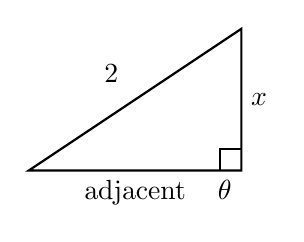
\begin{tikzpicture}[scale=0.9]
            \draw[thick] (0,0) -- (3,0) -- (3,2) -- cycle;
            \draw[thick] (2.7,0) -- (2.7,0.3) -- (3,0.3);
            \node[below] at (1.5,0) {adjacent};
            \node[right] at (3,1) {$x$};
            \node[above left] at (1.4,1.1) {$2$};
            \node[below left] at (3,0) {$\theta$};
        \end{tikzpicture}
        \end{center}
        }

        % Step 12.5
        \solutionStep{1}{Find the adjacent side}{
        \[
        \hspace*{-4em}
        \begin{array}{@{}r@{\hspace{1.25em}}l@{}}
        \text{By the \qdeflink{pyth-thm}{Pythagorean Theorem},}
        &
        \text{adjacent}=\sqrt{\text{hypotenuse}^2-\text{opposite}^2}
        \\[1.2ex]
        \text{Substitute the values}
        &
        \text{adjacent}=\sqrt{2^2-x^2}=\colorbox{yellow}{$\sqrt{4-x^2}$}
        \end{array}
        \]
        }

        % Step 12.6
        \solutionStep{1}{Find $\tan\theta$}{
        \[
        \hspace*{-4em}
        \begin{array}{@{}r@{\hspace{1.25em}}l@{}}
        \text{Use } \tan\theta=\frac{\text{opposite}}{\text{adjacent}}
        &
        \tan\theta=\frac{\colorbox{yellow}{$x$}}{\colorbox{yellow}{$\sqrt{4-x^2}$}}
        \end{array}
        \]
        }
        
        % Step 13
        \mainStep{1}{Write the final answer and choose the correct option.}
        
        % Step 13.1
        \solutionStep{1}{Substitute back}{
        \[
        \hspace*{-10em}
        \begin{array}{@{}r@{\hspace{1.25em}}l@{}}
        \text{From \hyperref[a-1:10.2]{Step 10.2},}
        &
        \displaystyle\int \frac{x^2}{(4-x^2)^{\frac{3}{2}}}\,dx
        =
        \tan\theta-\theta+C
        \\[1.2ex]
        \text{Substitute \hyperref[a-1:11.2]{Step 11.2} and \hyperref[a-1:11.6]{Step 11.6}}
        &
        \displaystyle\int \frac{x^2}{(4-x^2)^{\frac{3}{2}}}\,dx
        =
        \colorbox{yellow}{$\frac{x}{\sqrt{4-x^2}}$}
        -
        \colorbox{yellow}{$\sin^{-1}\!\left(\frac{x}{2}\right)$}
        + C
        \end{array}
        \]
        }
        
        % Step 13.2
        \solutionStep{1}{Final answer}{
        \[
        \text{The correct option is } \colorbox{yellow}{$\text{b}$}.
        \]
        }
        
       
    \end{tcolorbox}

    \newpage
    \section*{Definitions and Notation}

    \defanchor{antiderivative}\backtoterm{antiderivative}{Antiderivative}

    \textbf{Definition:}
    An antiderivative of a function is another function whose derivative gives back the original function.
    In simple words: if you take the derivative of the new function, you return to the old one.

    \textbf{Example:}
    \[
    \frac{d}{dx}\left(\frac{x^3}{3}\right)=x^2,
    \]
    so one antiderivative of $x^2$ is $\frac{x^3}{3}$.

    \defanchor{denominator}\backtoterm{denominator}{Denominator}

    \textbf{Definition:}
    In a fraction $\frac{p(x)}{q(x)}$, the denominator is the bottom part, $q(x)$.

    \textbf{Example:}
    \[
    \frac{x^2}{(4-x^2)^{3/2}}
    \]
    has numerator $x^2$ and denominator $(4-x^2)^{3/2}$.

    \defanchor{numerator}\backtoterm{numerator}{Numerator}

    \textbf{Definition:}
    In a fraction $\frac{p(x)}{q(x)}$, the numerator is the top part, $p(x)$.

    \textbf{Example:}
    \[
    \frac{x^2}{(4-x^2)^{3/2}}
    \]
    has numerator $x^2$.

    \defanchor{constant}\backtoterm{constant}{Constant}

    \textbf{Definition:}
    A constant is a fixed, unchanging value or number, such as $5$, $-10$, or $\pi$, that remains the same throughout a specific expression, equation, or function.

    \textbf{Example:}
    In
    \[
    3x+7,
    \]
    the $7$ is the constant term.

    \defanchor{variable}\backtoterm{variable}{Variable}

    \textbf{Definition:}
    A variable is a symbol, typically written in a lowercase letter like $x$, $y$, or $z$, that represents an unknown numerical value or a quantity that can change.

    \textbf{Example:}
    In
    \[
    3x+7,
    \]
    the $x$ is the variable.

    \defanchor{prod-power}\backtoterm{prod-power}{Power of a Product Rule}

    \textbf{Definition:}
    When raising a product of terms to a power, apply that power to each factor inside the parentheses, expressed as
    \[
    (ab)^n = a^n b^n.
    \]

    \textbf{Example:}
    \[
    (3x)^2=3^2x^2=9x^2.
    \]

    \defanchor{trig-sub}\backtoterm{trig-sub}{Trigonometric Substitution}

    \textbf{Definition:}
    Trigonometric substitution is a method for simplifying integrals with square roots by replacing $x$
    with a trig expression involving an angle.

    \textbf{Example:}
    \[
    \sqrt{4-x^2}=\sqrt{2^2-x^2}
    \]
    matches the pattern $\sqrt{a^2-x^2}$, so we use $x=2\sin\theta$.

    \textbf{Common patterns:}
    \[
    \sqrt{a^2-x^2}: x=a\sin\theta,\qquad
    \sqrt{a^2+x^2}: x=a\tan\theta,\qquad
    \sqrt{x^2-a^2}: x=a\sec\theta.
    \]

    \defanchor{frac-exp}\backtoterm{frac-exp}{Fractional Exponents}

    \textbf{Definition:}
    Fractional exponents rewrite powers as roots.
    \[
    a^{m/n}=\sqrt[n]{a^m}=\left(a^{1/n}\right)^m.
    \]

    \textbf{Example:}
    \[
    (4-x^2)^{3/2}=\left((4-x^2)^{1/2}\right)^3=\left(\sqrt{4-x^2}\right)^3.
    \]
    This means the $3/2$ power tells us to take a square root first, then cube.

    \defanchor{notation}\backtoterm{notation}{Square of Trigonometric Functions}

    \textbf{Definition:}
    \[
    (\sin\theta)^2=\sin^2\theta,\qquad
    (\cos\theta)^2=\cos^2\theta,\qquad
    (\tan\theta)^2=\tan^2\theta.
    \]

    \defanchor{pyth-id}\backtoterm{pyth-id}{Pythagorean Identity}

    \textbf{Definition:}
    The Pythagorean identity is the trig fact
    \[
    \sin^2\theta+\cos^2\theta=1
    \quad\Longleftrightarrow\quad
    1-\sin^2\theta=\cos^2\theta.
    \]

    \textbf{Example:}
    \[
    4-4\sin^2\theta=4(1-\sin^2\theta)=4\cos^2\theta.
    \]

    \defanchor{pyth-thm}\backtoterm{pyth-thm}{Pythagorean Theorem}

    \textbf{Definition:}
    In a right triangle with legs $a$ and $b$ and hypotenuse $c$,
    \[
    a^2+b^2=c^2.
    \]

    \textbf{Example:}
    If the hypotenuse is $2$ and one side is $x$, then the other side satisfies
    \[
    \text{adjacent}^2=2^2-x^2=4-x^2.
    \]

    \defanchor{square-root}\backtoterm{square-root}{Square Root}

    \textbf{Definition:}
    \[
    y^2=x
    \quad\Longrightarrow\quad
    y \text{ is a square root of } x.
    \]
    For nonnegative real numbers,
    \[
    \sqrt{x}=y
    \quad\Longleftrightarrow\quad
    y^2=x \text{ and } y\ge 0.
    \]

    \textbf{Example:}
    \[
    \sqrt{9}=3
    \]
    because
    \[
    3^2=9.
    \]

    \textbf{Key Properties:}
    \[
    \sqrt{x^2}=|x|
    \]
    \[
    \defanchor{sqrt-rule}\sqrt{a}\sqrt{b}=\sqrt{ab}
    \]
    \[
    \sqrt{\frac{a}{b}}=\frac{\sqrt{a}}{\sqrt{b}}
    \]
    \[
    \left(\sqrt{a}\right)^2=a
    \quad\text{and}\quad
    a^\frac{1}{2}=\sqrt{a}
    \]

    \defanchor{const-mult}\backtoterm{const-mult}{Constant Multiple Rule}

    \textbf{Definition:}
    When taking a derivative, a constant factor can stay in front:
    \[
    \frac{d}{d\theta}\bigl(c\,f(\theta)\bigr)=c\,f'(\theta).
    \]

    \textbf{Example:}
    \[
    \frac{d}{d\theta}(2\sin\theta)=2\cos\theta.
    \]

    \defanchor{add-int}\backtoterm{add-int}{Additive Property of Integrals}

    \textbf{Definition:}
    The integral of a sum or difference can be split into separate integrals:
    \[
    \int (f(x)+g(x))\,dx=\int f(x)\,dx + \int g(x)\,dx
    \]
    and
    \[
    \int (f(x)-g(x))\,dx=\int f(x)\,dx - \int g(x)\,dx.
    \]

    \textbf{Example:}
    \[
    \int (\sec^2\theta-1)\,d\theta
    =
    \int \sec^2\theta\,d\theta-\int 1\,d\theta.
    \]

    \defanchor{abs-val}\backtoterm{abs-val}{Absolute Value}

    \textbf{Definition:}
    The absolute value of a number is its distance from $0$, so it is never negative.

    \textbf{Example:}
    \[
    |3|=3,\qquad |-3|=3.
    \]
    In Q34 we use
    \[
    \sqrt{u^2}=|u|.
    \]
    Since $0\le \theta \le \frac{\pi}{2}$, we know $\cos\theta\ge 0$, so
    \[
    |\cos\theta|=\cos\theta.
    \]

    \defanchor{trig-ratios}\backtoterm{trig-ratios}{Basic Trig Ratios: Sine, Cosine, and Tangent}

    \textbf{Definition:}
    In a right triangle:
    \[
    \sin\theta=\frac{\text{opposite}}{\text{hypotenuse}},\qquad
    \cos\theta=\frac{\text{adjacent}}{\text{hypotenuse}},\qquad
    \tan\theta=\frac{\text{opposite}}{\text{adjacent}}.
    \]

    \textbf{Example:}
    If $\sin\theta=\frac{x}{2}$, then opposite $=x$ and hypotenuse $=2$.
    The adjacent side is
    \[
    \sqrt{2^2-x^2}=\sqrt{4-x^2},
    \]
    so
    \[
    \tan\theta=\frac{x}{\sqrt{4-x^2}}.
    \]

    \defanchor{inv-sine}\backtoterm{inv-sine}{Inverse Sine $\sin^{-1}(x)$}

    \textbf{Definition:}
    Also written $\arcsin(x)$, inverse sine returns the angle whose sine is $x$.

    \textbf{Example:}
    If $\sin\theta=\frac{x}{2}$, then
    \[
    \theta=\sin^{-1}\!\left(\frac{x}{2}\right).
    \]

\end{document}
